%----------------------------------------------------
% Setup Beamer
%----------------------------------------------------
\documentclass[hyperref={colorlinks=true}]{beamer}

%----------------------------------------------------
% Packages to use
%----------------------------------------------------
\input{../packages.sty}

%----------------------------------------------------
% Setup Theme
%----------------------------------------------------
\input{../theme.sty}

%----------------------------------------------------
% Table of Contents at each section transition
%----------------------------------------------------

\AtBeginSection[]
{
   \begin{frame}
       \frametitle{Outline}
       \setcounter{tocdepth}{2}
       \tableofcontents[currentsection]
   \end{frame}
}

%----------------------------------------------------
% Colors
%----------------------------------------------------
\input{../mycolors.sty}

%----------------------------------------------------
% Style, formatting, and new commands
%----------------------------------------------------
\newcommand{\CourseYear}   {2024}
\newcommand{\CanvasURL}    {https://canvas.uchicago.edu/courses/58627}
\newcommand{\CanvasLink}   {\href{\CanvasURL}{\CanvasURL}}
\newcommand{\GitHubURL}    {https://github.com/UChicagoPhysics/PHYS250}
\newcommand{\GitHubLink}   {\href{\GitHubURL}{\GitHubURL}}
\newcommand{\PlatformURL}  {https://binderhub.pile.uchicago.edu/}
\newcommand{\PlatformLink} {\href{\PlatformURL}{\PlatformURL}}
\newcommand{\PiazzaURL}    {https://canvas.uchicago.edu/courses/58627/discussion\_topics}
\newcommand{\PiazzaLink}   {\href{\PiazzaURL}{\PiazzaURL}}
\input{../newcommands.sty}
\input{../EandMcommands.sty}

%----------------------------------------------------
% Set paths for plots and images
%----------------------------------------------------
\input{../paths.sty}

%----------------------------------------------------
% SETTINGS FOR THIS LECTURE
%----------------------------------------------------
\newcommand{\lecnum }  {Lecture 15}
\newcommand{\lecdate}  {November 27, 2024}
\newcommand{\topic}    {Neural Networks -- Part I}

%-----------------------------------------------------------------------------------------
% Title: [Column]{Title}
%-----------------------------------------------------------------------------------------
\title[PHYS 250 (Autumn 2024) -- \lecnum]{\topic}

%-----------------------------------------------------------------------------------------
% SubTitle: [Column]{Subtitle}
%-----------------------------------------------------------------------------------------
\subtitle{PHYS 250 (Autumn 2024) -- \lecnum}

%-----------------------------------------------------------------------------------------
% Author: [SubAuthor]{Author}
%-----------------------------------------------------------------------------------------
\author[D.W.~Miller]{David Miller}

%----------------------------------------------------
% Institute: [SubInst]{Institute}
%----------------------------------------------------
\institute[EFI, Chicago] 
{
  Department of Physics and the Enrico Fermi Institute\\
  University of Chicago
}

%----------------------------------------------------
% Institute: [SubInst]{Institute}
%----------------------------------------------------
\date[\lecdate]{\lecdate}

\subject{PHYS 250 Lecture}

\begin{document}

%==========================================================================================
% TITLE PAGE
%==========================================================================================

{
\begin{frame}
  \titlepage
\end{frame}
}

%==========================================================================================
\section[Introduction to Neural Networks]{Introduction to Neural Networks}
%==========================================================================================

%-----------------------------------------------------------------------------------------
\subsection[Context of Machine Learning]{Context of Machine Learning}
%-----------------------------------------------------------------------------------------

\begin{frame}%[shrink=10]
  \frametitle{Machine learning generally}

  Machine learning is an area of study based broadly on developments in computer science over the past 50 years that aims to use \bluebf{algorithmic approaches to discovering, identifying, and analyzing, patterns of interest in datasets}.
  
  \begin{itemize}
    \item Key phrase here is \bluebf{algorithmic}
    \item We want \bluebf{models} that tell us something about a dataset
  \end{itemize}
   
  \begin{center} \Large \alertbf{Sounds like something we'd be interested in!} \end{center}
  
  \ra\ Definitely, but much broader concept here than just what we've been discussing so far in the course.

\end{frame}

%-----------------------------------------------------------------------------------------

\begin{frame}%[shrink=10]
  \frametitle{Machine learning applications}

  \setbeamercovered{transparent}

  What are we using these algorithms to \textit{do}?
  
  \mysp
  
  \begin{itemize}[<+->]
    \item \textbf{Supervised learning:} \bluebf{machine is presented examples of multiple classes and learns to differentiate} (\textit{discover known patterns on unknown data})
    \begin{itemize}
      \item \alertbf{Classification:} identify categories of variables; e.g. signal vs. background
      \item \alertbf{Regression:} estimate relationships among variables; e.g. calibration
      \item \alertbf{Generation:} generate a set of variables from a category (e.g. image)
    \end{itemize}
    \item \textbf{Unsupervised learning:} \bluebf{machine is presented data and asked to provide multiple classes} (\textit{discover unknown patterns on known data})
    \begin{itemize}
      \item \alertbf{Clustering:} grouping set of objects in a dataset; e.g. jets of hadrons
      \item \alertbf{Anomaly detection:} identifying rare events or observations; e.g. errors
    \end{itemize}
  \end{itemize}
  
  \begin{figure}
    \centering
    \includegraphics<1-2>[width=0.4\textwidth]{Classification.png}
    \includegraphics<3>[width=0.4\textwidth]{Regression.png}
    \includegraphics<4>[width=0.4\textwidth]{Generation.jpg}
    \includegraphics<5-6>[width=0.4\textwidth]{Clustering.png}
    \includegraphics<7>[width=0.3\textwidth]{Anomaly.png}
  \end{figure}


\end{frame}

%-----------------------------------------------------------------------------------------

\begin{frame}%[shrink=10]
  \frametitle{Where do neural networks fit in?}

  There are many \bluebf{tools} that we can use to \alertbf{learn} how to perform these tasks. 
  
  \mysp

  \begin{ucblock}{Neural networks}
  Neural networks provide a framework for non-linear fitting and parameter estimation with limited input data but for cases in which the input data are understood and the categories (for example) are known.  
  \end{ucblock}
  
  \mysp
    
  \begin{center} \bluebf{Neural networks are \underline{proven} to be ``universal approximators''} \end{center}
  
  See \href{https://doi.org/10.1016/0893-6080(91)90009-T}{Kurt Hornik, ``Approximation Capabilities of Multilayer Feedforward Networks'', Neural Networks, 4, 251-257 (1991)}.
  
  \mysp
  
  One straightforward way to think of this is as a composition of functions $f(\mathbb{A}\mathbf{x}+\mathbf{b})$ for inputs $\mathbf{x}$ (features) matrix $\mathbb{A}$ (weights), bias $\mathbf{b}$, non-linearity $f$. Given some data, the algorithm should tell us which of a pre-defined set of categories the data fall into, even if it's a complicated non-linear function that describes the boundary between these categories.

  
\end{frame}
  
%-----------------------------------------------------------------------------------------
\subsection[Motivations from the perspective of modeling]{Motivations from the perspective of modeling}
%-----------------------------------------------------------------------------------------

\begin{frame}%[shrink=10]
  \frametitle{Motivations for neural networks}

  If we can use a neural network to approximate any (incl. non-linear) function, then this is strong motivation for using it to learn complicated functions that describe classes of objects, potentially in high-dimensional spaces.

  \begin{figure}
    \centering
    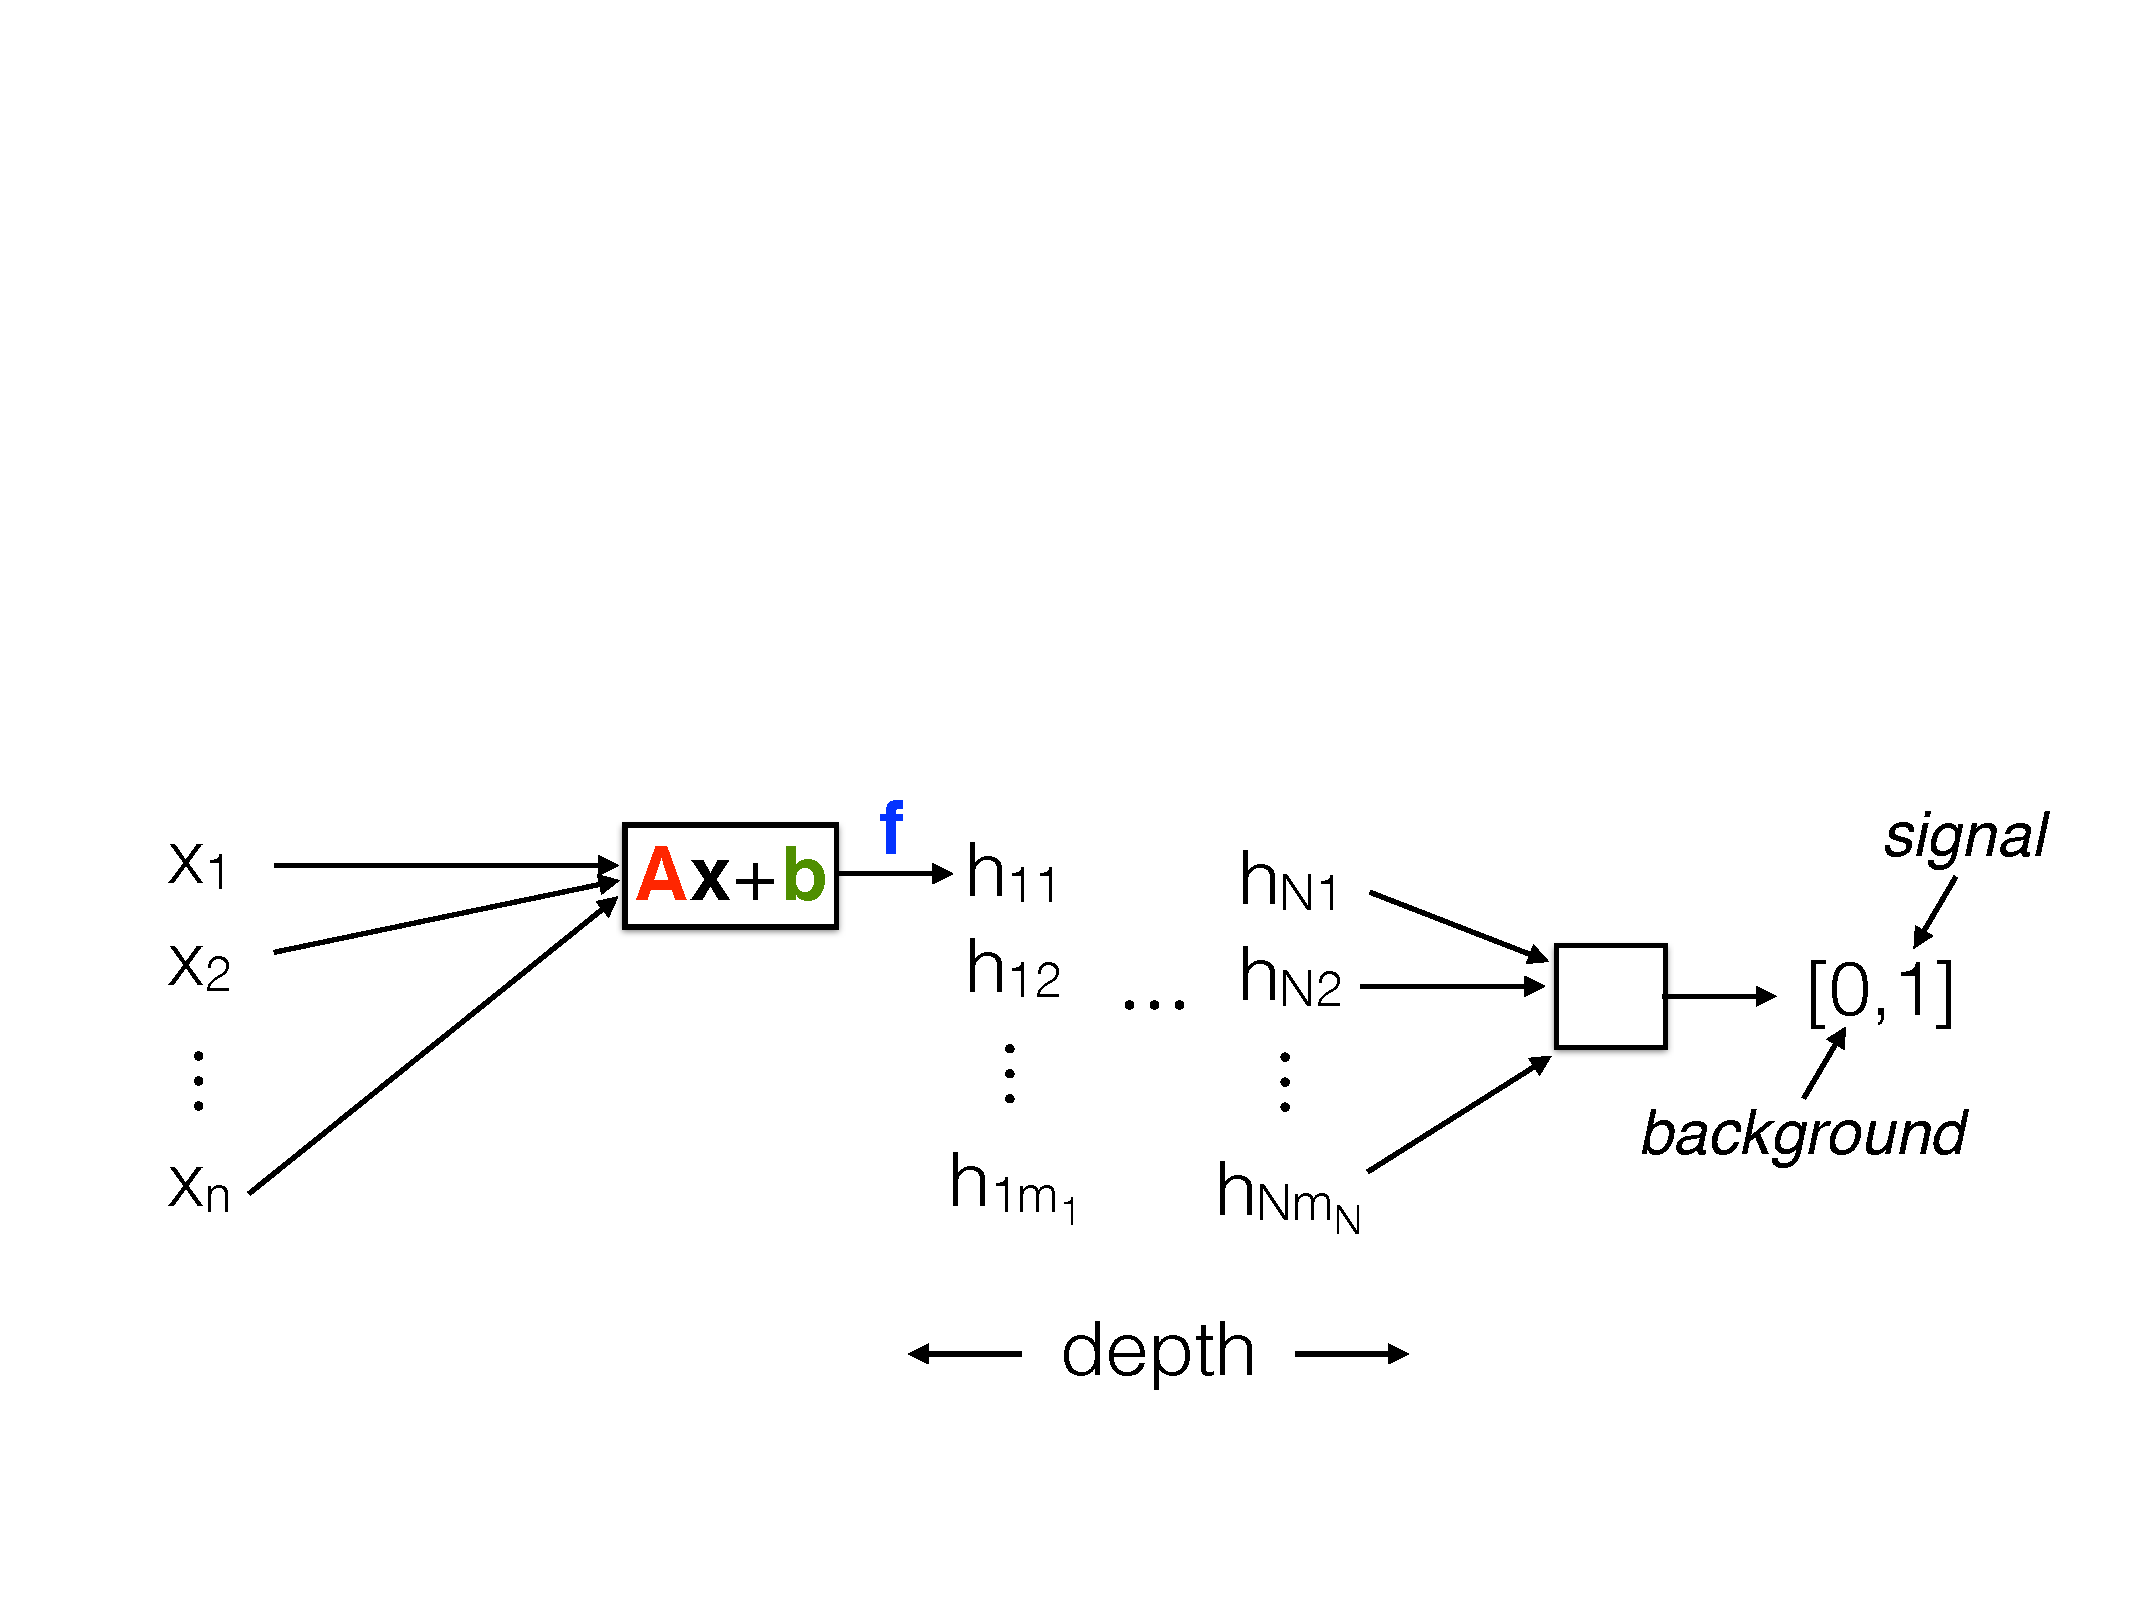
\includegraphics[width=0.9\textwidth]{SimpleNeuralNetwork.pdf}
  \end{figure}
  
  
\end{frame}

%-----------------------------------------------------------------------------------------

\begin{frame}%[shrink=10]
  \frametitle{Very, very naive strawman example}

  Suppose the ``function'' we want to learn is to map kilometers\ra\ miles. 
  
  \mysp
  
  Given a \alertbf{``training dataset''} of input and output pairs, we can test a simple function with a parameter the defines the conversion, and then \bluebf{iteratively update} the parameters based on how far from the \alertbf{``true''} value we end up.

  \begin{figure}
    \centering
    \includegraphics<1>[width=0.7\textwidth]{km-to-mi-1.png}%
    \includegraphics<2>[width=0.8\textwidth]{km-to-mi-2.png}%
    \includegraphics<3>[width=0.8\textwidth]{km-to-mi-3.png}%
    \includegraphics<4>[width=0.8\textwidth]{km-to-mi-4.png}%
    \includegraphics<5>[width=0.8\textwidth]{km-to-mi-5.png}%
\end{figure}
  
  Obviously, we want to extend this to non-linear cases.
  
\end{frame}


%-----------------------------------------------------------------------------------------
\subsection[Motivations from the perspective of biology]{Motivations from the perspective of biology}
%-----------------------------------------------------------------------------------------

%-----------------------------------------------------------------------------------------

\begin{frame}%[shrink=10]
  \frametitle{The biological model}

  The way brains work is by establishing connections between various neurons.
  
  \mysp
  
  Once connections are made, initial stimuli give similar (though not always identical) results
  
  \begin{figure}
    \centering
    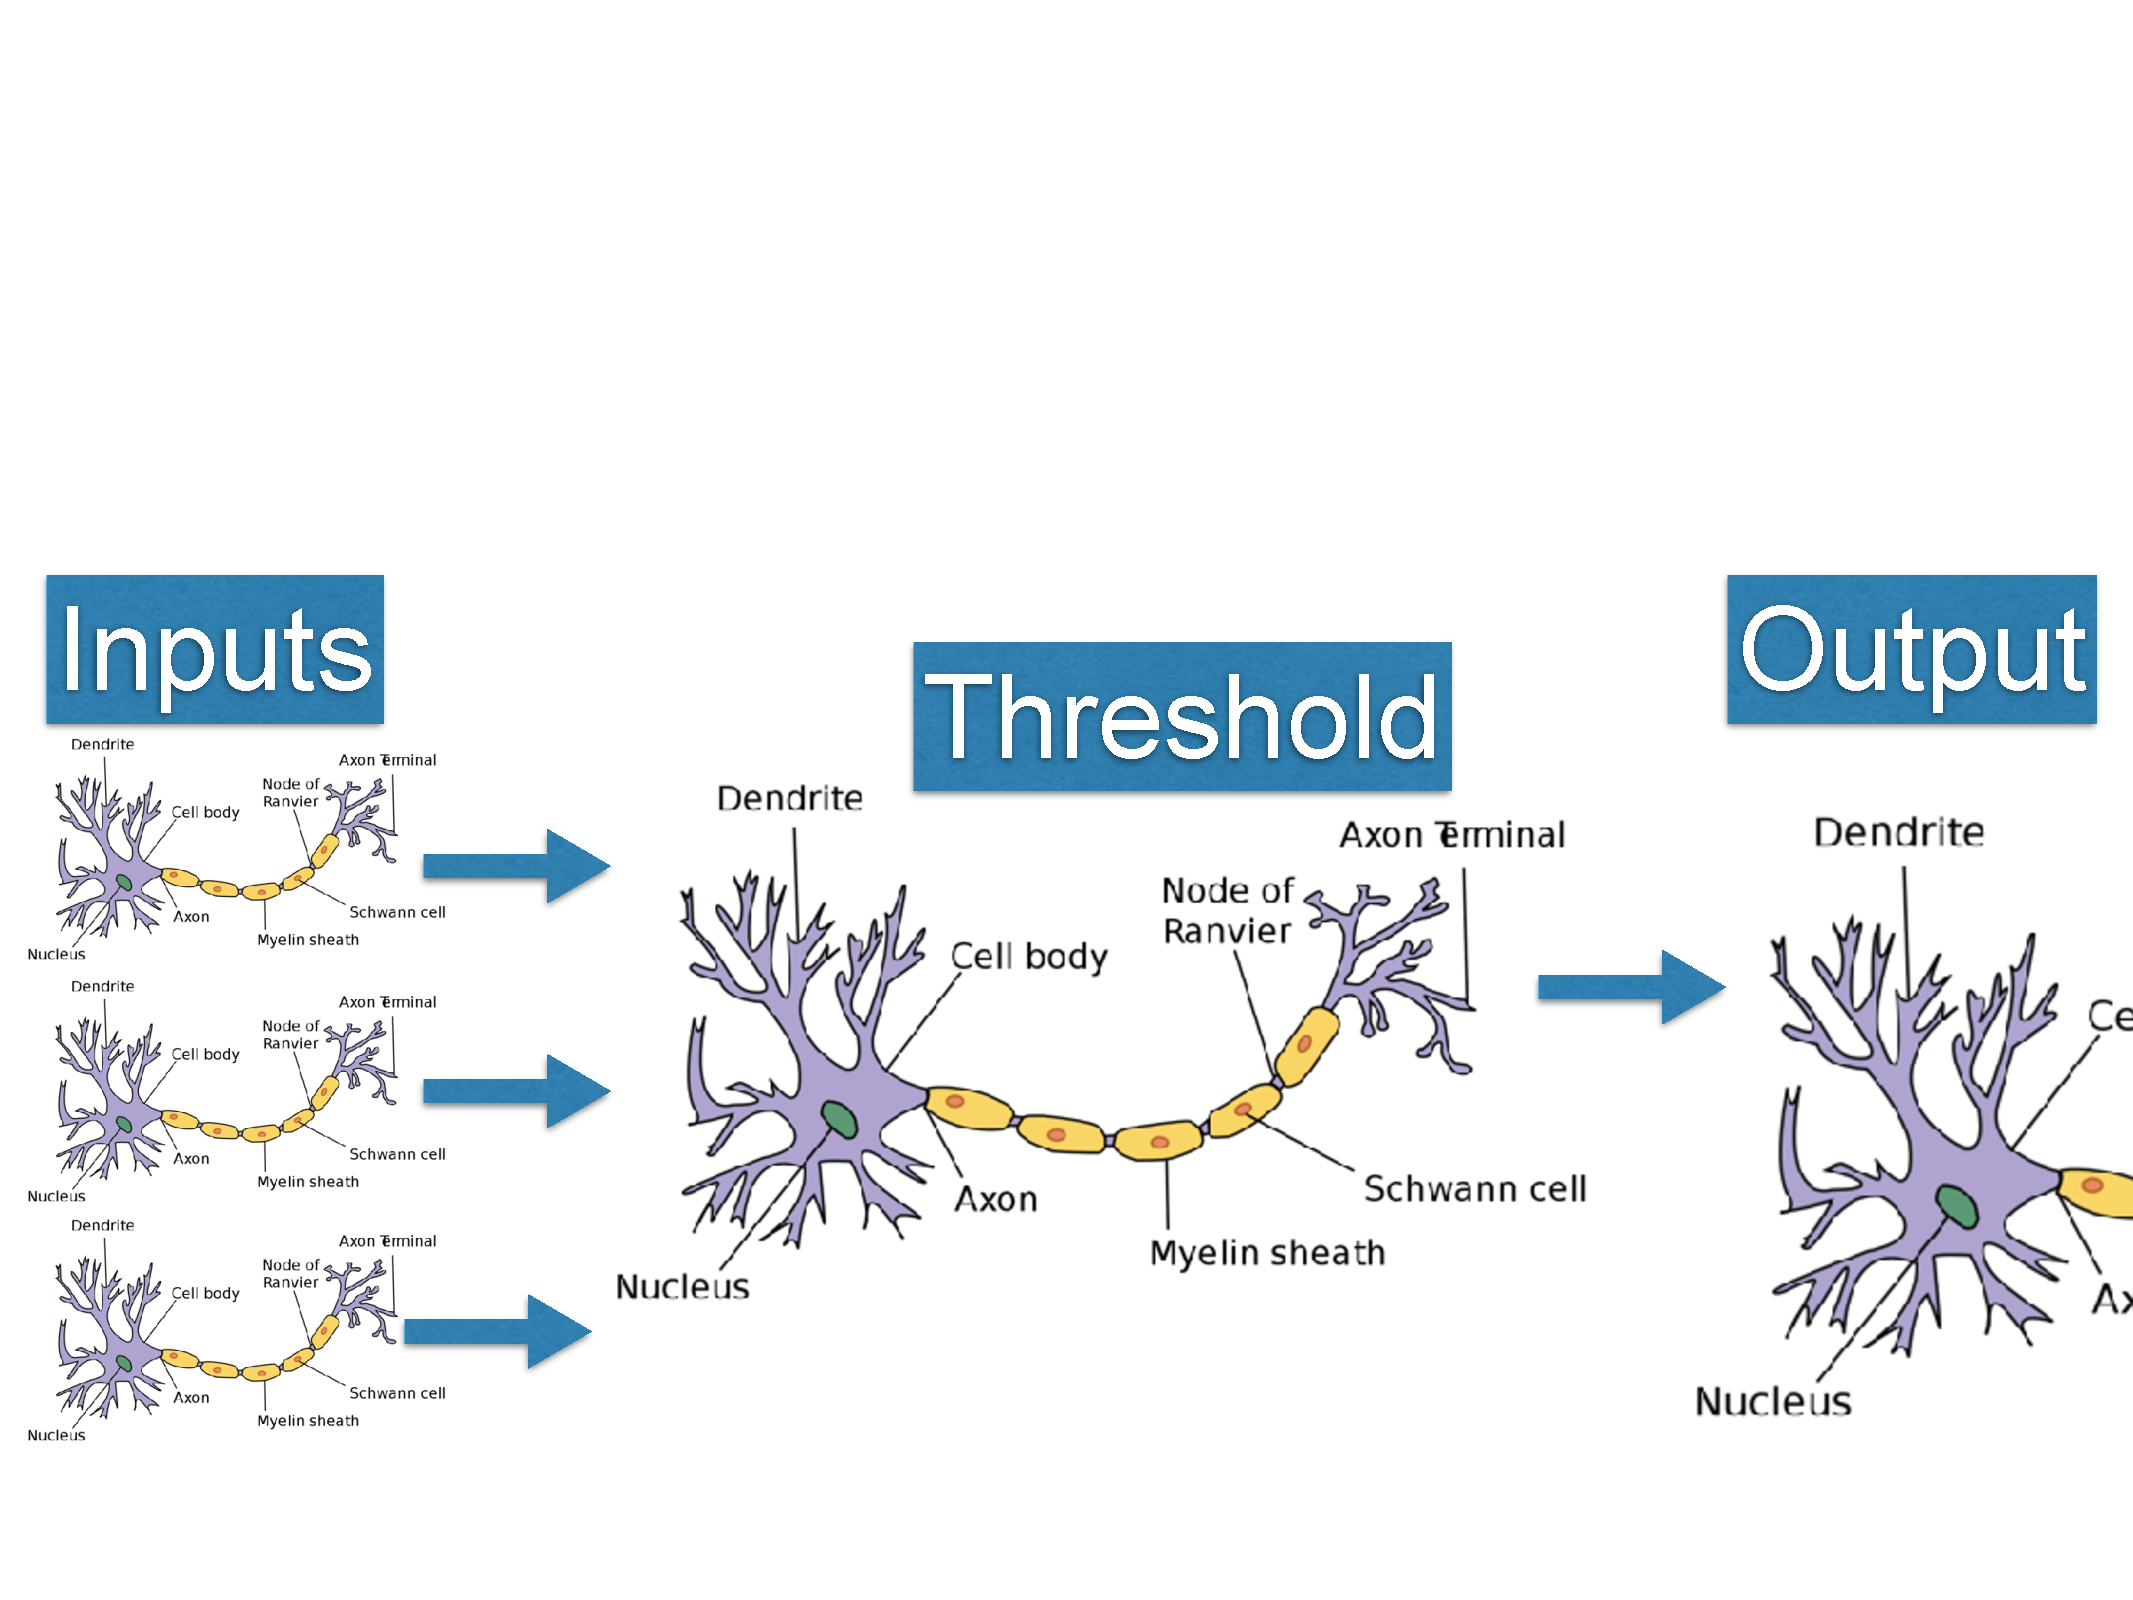
\includegraphics[width=0.95\textwidth]{NeuronModel.pdf}%
\end{figure}
    
\end{frame}

%-----------------------------------------------------------------------------------------

\begin{frame}%[shrink=10]
  \frametitle{Artificial neuron model}

  McCulloch and Pitts (1943) model of a single neuron. Rosenblatt (1958) then developed the \bluebf{ perceptron} based on this, the oldest neural network still in use today; provided an algorithm to train the perceptron network, built it in electronics, and proved convergence in linearly separable case.
  
  \mysp
    
  \begin{figure}
    \centering
    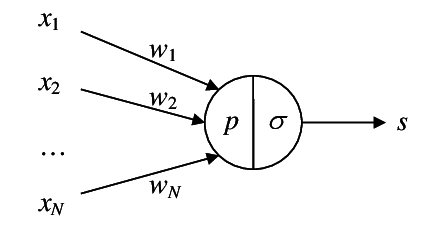
\includegraphics[width=0.45\textwidth]{The-McCulloch-and-Pitts-1943-model-of-a-single-neuron-Source-Adapted-from-Franck.png}%
    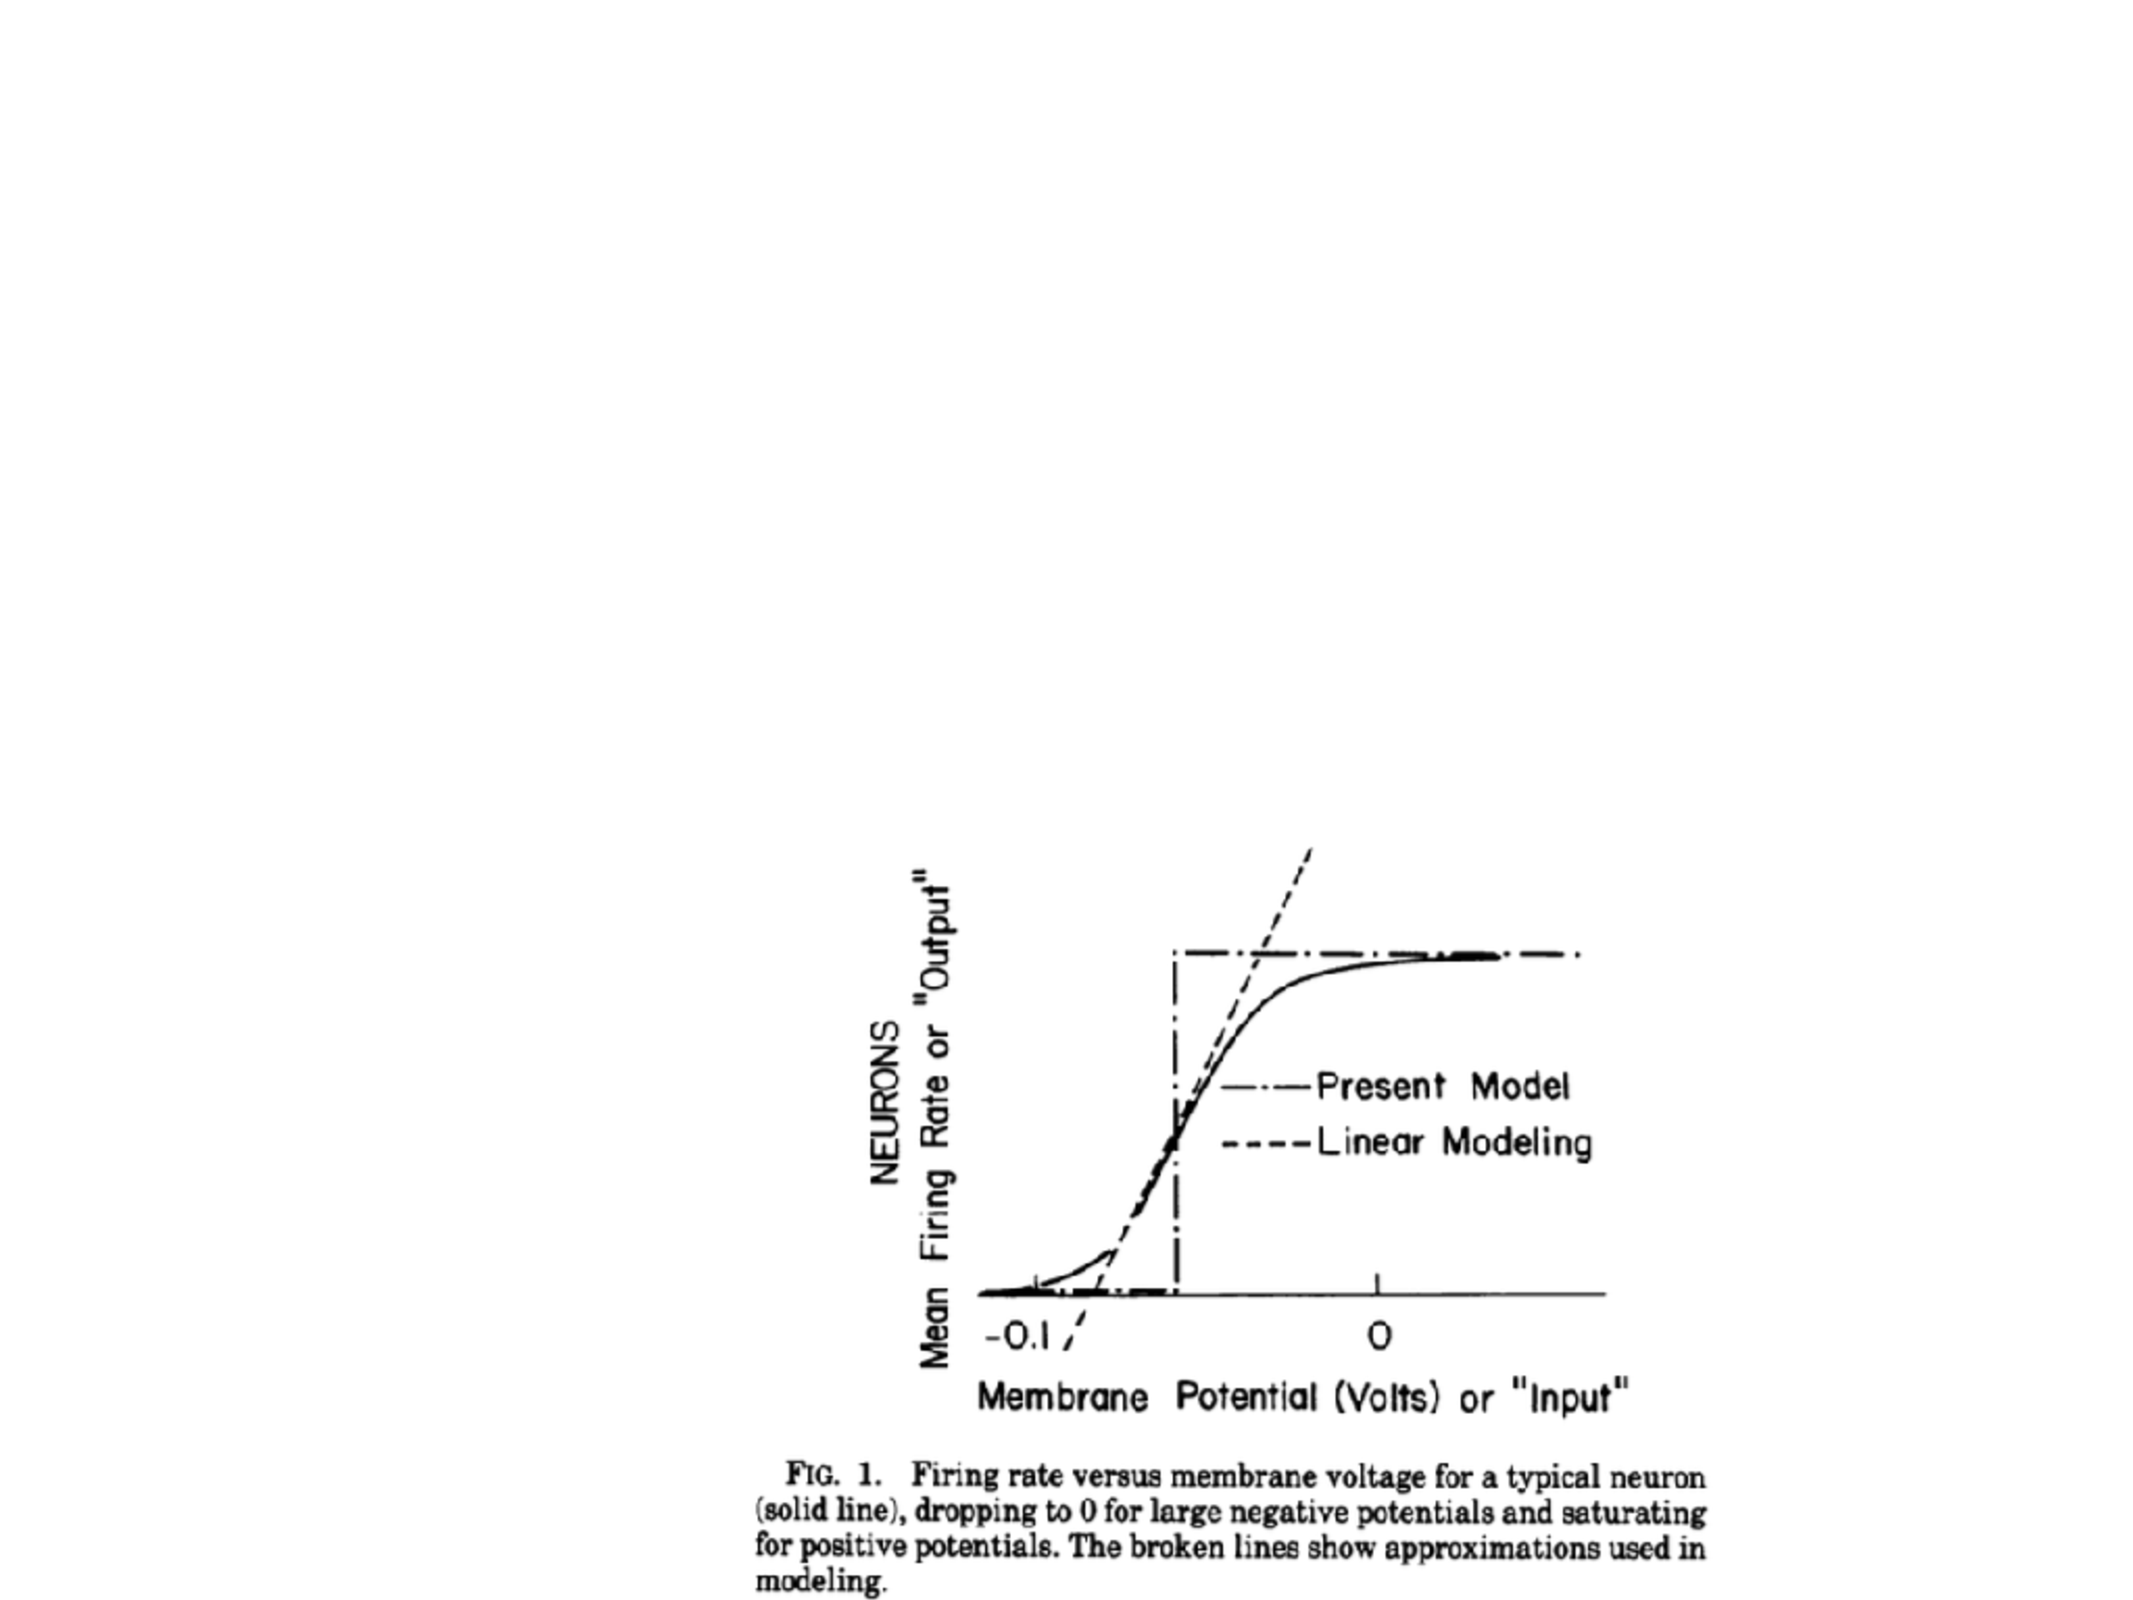
\includegraphics[width=0.45\textwidth]{PittsModel.pdf}%
\end{figure}
    
\end{frame}



%-----------------------------------------------------------------------------------------
\subsection[Discussion of applications]{Discussion of applications}
%-----------------------------------------------------------------------------------------

%-----------------------------------------------------------------------------------------

\begin{frame}%[shrink=10]
  \frametitle{Neural networks are, maybe literally, everywhere}

    
  \begin{figure}
    \centering
    \includegraphics<1>[width=0.95\textwidth]{NNs-1.png}%
    \includegraphics<2>[width=0.95\textwidth]{NNs-2.png}%
    \includegraphics<3>[width=0.95\textwidth]{NNs-3.png}%
    \includegraphics<4>[width=0.95\textwidth]{QuarksGluons.pdf}%
\end{figure}
    
\end{frame}


%==========================================================================================
\section[Foundations of Neural Networks]{Foundations of Neural Networks}
%==========================================================================================

%-----------------------------------------------------------------------------------------
\subsection[Activation functions]{Activation functions}
%-----------------------------------------------------------------------------------------

\begin{frame}%[shrink=10]
  \frametitle{Activation functions}

  We need a network that can effectively learn a complex function by weighting the individual outputs of each node.  
    
  \begin{figure}
    \centering
    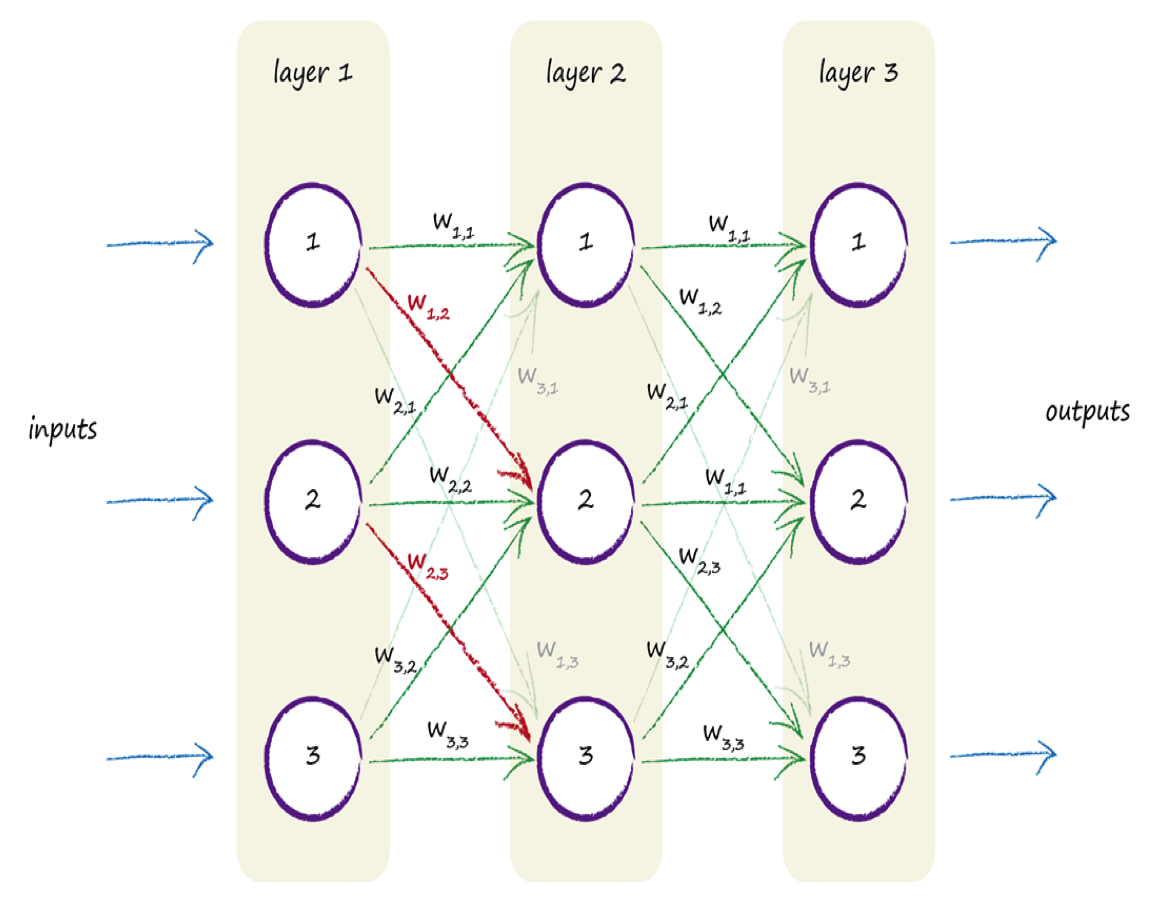
\includegraphics[width=0.75\textwidth]{NN-2layer.png}%
  \end{figure}
    
\end{frame}




%-----------------------------------------------------------------------------------------

\begin{frame}%[shrink=10]
  \frametitle{Non-linearity functions for learning}

  This is the function that defines the output of a node. Typically, we want to map the resulting values into a range between $[0, 1]$, or  $[-1,1]$
    
  \begin{figure}
    \centering
    \includegraphics<1>[width=0.85\textwidth]{NonLinearFunction.pdf}%
    \includegraphics<2>[width=0.85\textwidth]{NonLinearFunction-2.pdf}%
  \end{figure}
    
\end{frame}


%-----------------------------------------------------------------------------------------
\subsection[Training]{Training}
%-----------------------------------------------------------------------------------------

%-----------------------------------------------------------------------------------------

\begin{frame}%[shrink=10]
  \frametitle{Training a neural network}

  The \bluebf{``objective function''} is minimized using \alertbf{``stochastic gradient decent''}:
  \begin{itemize}
    \item iterative method for optimizing the ``loss'' or the error that we are trying to minimize 
  \end{itemize}
    
  \begin{figure}
    \centering
    \includegraphics<1>[width=0.75\textwidth]{Training.pdf} \\
  \end{figure}
    
\end{frame}

%-----------------------------------------------------------------------------------------

\begin{frame}%[shrink=10]
  \frametitle{Back-propagation}

  For the matrix that defines the \alertbf{weights} we want to update those weights based on 
    
  \begin{figure}
    \centering
    \includegraphics<1>[width=0.85\textwidth]{Learning.pdf} 
  \end{figure}
    
  Here, \bluebf{back-propagation} is shorthand for ``the backward propagation of errors'' since an error is computed at the output and distributed backwards throughout the network's layers.
  
  \mysp
  
  Really, \bluebf{back-propagation} is \textbf{just a special case of computational differentiation!}. 
    
\end{frame}

%-----------------------------------------------------------------------------------------

\begin{frame}%[fragile, shrink=20]
  \frametitle{Back-propagation}

  Phase 1: propagation
  \begin{itemize}
    \item Propagation forward through the network to generate the output value(s)
    \item Calculation of the cost (error term)
    \item Propagation of the output activations back through the network using the training pattern target to generate the deltas (the difference between the targeted and actual output values) of all output and hidden neurons.
  \end{itemize}

  Phase 2: weight update

  \begin{itemize}
    \item The weight's output delta and input activation are multiplied to find the gradient of the weight.
    \item A ratio (percentage) of the weight's gradient is subtracted from the weight.
  \end{itemize}

This ratio (percentage) influences the speed and quality of learning; it is called the learning rate ($\eta$ on the previous slide). The greater the ratio, the faster the neuron trains, but the lower the ratio, the more accurate the training is. The sign of the gradient of a weight indicates whether the error varies directly with, or inversely to, the weight. Therefore, the weight must be updated in the opposite direction, ``descending'' the gradient. 

  \begin{figure}
    \centering
    \includegraphics<1>[width=0.99\textwidth]{Pseudocode.png} 
  \end{figure}
 
  
    
\end{frame}

%-----------------------------------------------------------------------------------------

\begin{frame}%[fragile, shrink=20]
  \frametitle{Training and validation}

  \begin{figure}
    \centering
    \includegraphics<1>[width=0.99\textwidth]{Validation.pdf} 
  \end{figure}
 
  
    
\end{frame}



  
%==========================================================================================
%==========================================================================================
\end{document}
